\section{Localisation}
\label{section:workflow:localisation}

So far, we have assessed our code as more or less one big black box.

\begin{itemize}
  \item We did not ask \emph{which part of the code} causes a problem. 
  \item We did not ask \emph{when} it arises throughout the execution.
  \item We did not ask \emph{where}, i.e.~on which rank (if we run over multiple
  nodes) a problem arises.
  \item We distinguished, to some degree, \emph{what} we want to study in our
  code, i.e.~which quantity of interest.
\end{itemize}


\noindent
The importance of the four dimensions strongly depends on what we are interested in and what we are investigating:
Single-core flaws imply that the ``where'' question does not play a significant role.
Inter-node flaws might suggest that the ``where'' question is the primary concern to address.
Not all four dimensions are always equally important.


\subsection{Tool support}

To assess the code and dive deeper into details, it makes sense to zoom into details along these four dimensions to manage complexity.
For this, most tools provide features. 
We broadly distinguish two approaches:
Tools allow us to \emph{explore and zoom} into data after the collection, i.e.~to explore the gathered data space, while \emph{filter mechanisms} allow the assessor to record only specific information right from the start.
Obviously, an a posteriori approach is superior in the sense that we do not run risk that we ``forgot'' to record data initially.
However, the sheer amount of data recorded by many tools often make it necessary to define filters beforehand.

\subsubsection{Filtering}

To filter data, most toolchains provide marker APIs.
Alternatively, they come along with precompilers which take your code and add the filter on/off statements to it before it is passed on to the compiler.
Some very popular tools are sketched in Chapter~\ref{chapter:tools}, including the APIs they offer.


\subsubsection{Zoom in}


\begin{instructions}{\vtune}
 \vtune~offers in almost all tabs an overview over the temporal behaviour at the bottom which splits up the observations over cores.
 A right click or drawing an observation interval allows you to zoom in.  
\end{instructions}

 %% this an old VTune box from the 'Preparation' Chapter
%\begin{instructions}{\vtune}
%Start a multithreaded run and mark the actual computational phase in the timeline at the bottom.
%Switch to the \emph{Bottom up} view.
%\emph{Zoom in and filter by selection} will narrow down the profile to the region of interest.
%Sort by \emph{Effective Time} and change to \emph{Show Data As \ldots~Percentage}.
%Make notes of all the entries above roughly 1\% (rule of thumb) and/or track the top 10 routines. 
%\end{instructions}

\subsection{Labelling of code parts}

Software typically contains quite a lot of boilerplate code: 
predominantly administrative routines that enable calculations but don't deliver actual science flops. 
For several follow-on exercises, it will be very useful to know which code parts deliver science and which code parts do not directly add scientific value.
This is domain knowledge.
Using it contradicts, to some degree, our ambition to run a performance assessment in a black-box manner.


However, we do not ask an assessor to understand what a code does.
We require the assessor to know which code parts contribute towards the science case.
For this reason, it is absolutely sufficient to hand a first profile back to a domain expert and to ask them to label those routines that do the actual calculations. 

As an example: 
In a linear algebra code, the actual matrix-vector products, scalar products, \ldots~all deliver science.
The allocations for temporary block matrices, the exchange routines for rows of the matrices, any indexing over the sparsity pattern, and so forth do not contribute calculations.
They are absolutely essential, but they do not give us the MFlops/s.


As your analysis progresses, you might run into situations where functions suddenly appear to be hot that you have not seen before.
In this case, you can kind of safely assume that these functions do \emph{not} contribute to the science directly.
If they didn't show up for a small-scale, few-core run, then they likely do not feed directly into the result.


\paragraph*{How it works}

\begin{itemize}[noitemsep]
  \item[$\boxplus$] Upon your very first profiling, ask a code expert which code parts (functions) actually perform calculations, i.e.~contribute towards the science.
\end{itemize}


\paragraph*{How it does not work}

\begin{itemize}[noitemsep]
  \item[$\boxminus$] Assume that all routines deliver science (even though you may assume that all are necessary).
\end{itemize}


\subsection{Related work}

\begin{figure}
 \begin{center}
  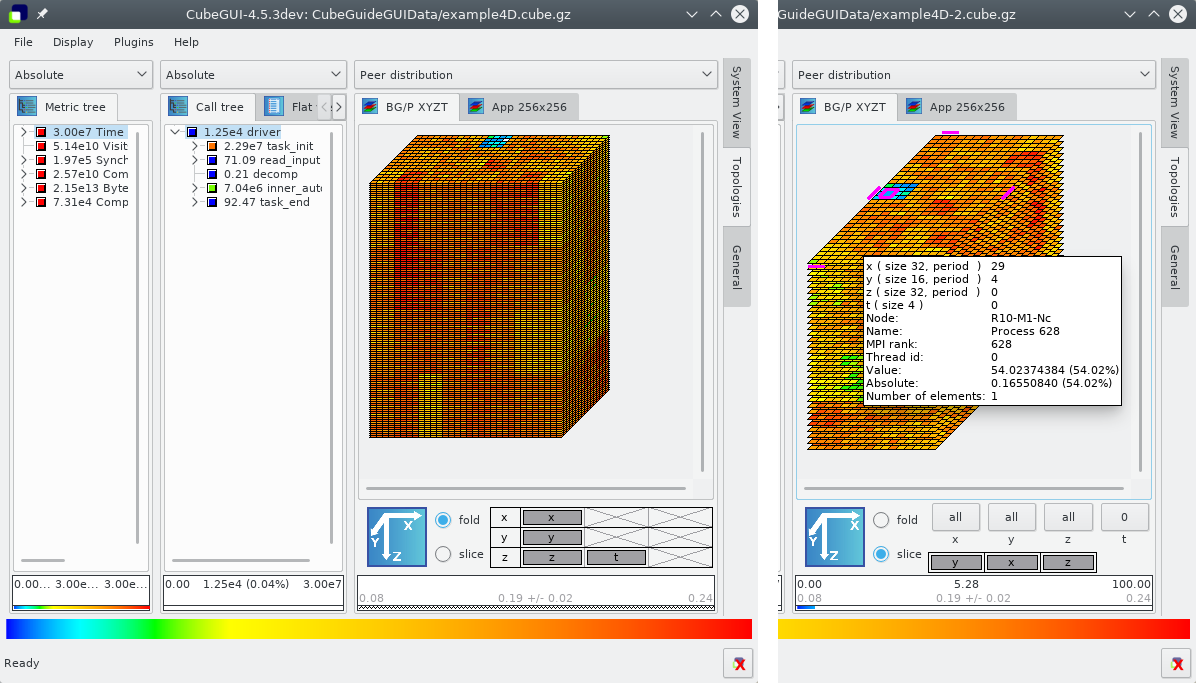
\includegraphics[width=0.7\textwidth]{workflow/cube-gui.png}
 \end{center}
 \caption{
  Screenshot of the CubeGUI from the tool's webpage.
  \label{figure:workflow:localisation:cube-gui}
 }
\end{figure}

Our four rubrics are strongly inspired by the CubeGUI work\footnote{\url{https://helmholtz.software/software/cubegui}}:
In this graphical front-end, which is used, among others, by the Scalasca tool, users can study effects along the dimensions
metric, call tree/graph, and system (Figure~\ref{figure:workflow:localisation:cube-gui}).


The metric corresponds to the hypotheses discussed in the following deep-dive sections.
They are picked up in the subsequent section, too.
If you plan to study a particular hypothesis which corresponds directly to a CUBE metric, the tool becomes particularly useful.
call tree/graph is a the so-called program dimension and allows users to study where certain flaws result from, i.e.~which code parts cause the pain.
The system dimension finally helps users to filter along the where dimension. 


We propose to extend the three-dimensional analysis from CubeGUI by a temporal dimension for most analyses,
which is implicitly supported by Cube by filtering data production a priori
or by embedding certain code parts into markers such that the active code sections can be distinguished.  


\subsection{Take away}

The most frequent quantity of interest (metric) to developers is typically how much time is spent in routines and which routines or function calls are to be blamed for some behaviour.
The routines consuming most time are called \emph{hotspots} of a code.
This section's rationale is that hotspots are important, but simply looking at a profile and picking out the most expensive routine does not provide all data required for HPC workloads.
Massivel load imbalanced for example will manifest in totally misleading results on undersubscribed nodes, while the profile on the oversubscribed node will maybe not even suggest that it causes issues. 

This chapter thus makes a few simple suggestions:

\begin{enumerate}
  \item Focus on the smallest relevant time scale of a program run (e.g.~study only one iteration of an iterative solver),
  \item narrow down the amount of code you consider (i.e.~look at the top hotspots only),
  \item measure only on a few characteristics nodes or cores, 
  \item and always consider the effect first.
\end{enumerate}

\noindent
That is, we suggest to invert the analysis flow:
We define which effect we are interested in, and narrow down the search space taking the effect of interest into account.


\paragraph*{How it works}

\begin{itemize}[noitemsep]
  \item[$\boxplus$] Once you have a first high-level overview, always use a tool to find out if the effects of interest are spatially and temporally localised.
  \item[$\boxplus$] Focus as much as possible.
  \item[$\boxplus$] Adopt the search space to the effect you are after, i.e.~the hypotheses you are studying.
\end{itemize}


\paragraph*{How it does not work}

\begin{itemize}[noitemsep]
  \item[$\boxminus$] Start with some hotspot analysis.
  \item[$\boxminus$] Jump straight into some traces or profiles without spending time to
  think what metrics and program parts are relevant to answer your
  hypotheses regarding  performance flaws.
  \item[$\boxminus$] Draw conclusions from global observations on all code parts
  and compute resources (cores or ranks).
\end{itemize}
